\documentclass[usenatbib]{mn2e}

\usepackage[toc,page]{appendix}
\usepackage{amsmath, amssymb}
\usepackage{bm}% bold math
\usepackage{cancel, caption}
\usepackage{dcolumn}% Align table columns on decimal point
\usepackage{epsfig, epsf}
\usepackage{graphicx,fancyhdr,natbib,subfigure}
\usepackage{lscape, longtable}
\usepackage{hyperref,ifthen}
\usepackage{verbatim}
\usepackage{color}
\usepackage[usenames,dvipsnames]{xcolor}
\usepackage{listings}
%% http://en.wikibooks.org/wiki/LaTeX/Colors



%%%%%%%%%%%%%%%%%%%%%%%%%%%%%%%%%%%%%%%%%%%
%       define Journal abbreviations      %
%%%%%%%%%%%%%%%%%%%%%%%%%%%%%%%%%%%%%%%%%%%
\def\nat{Nat} \def\apjl{ApJ~Lett.} \def\apj{ApJ}
\def\apjs{ApJS} \def\aj{AJ} \def\mnras{MNRAS}
\def\prd{Phys.~Rev.~D} \def\prl{Phys.~Rev.~Lett.}
\def\plb{Phys.~Lett.~B} \def\jhep{JHEP} \def\nar{NewAR}
\def\npbps{NUC.~Phys.~B~Proc.~Suppl.} \def\prep{Phys.~Rep.}
\def\pasp{PASP} \def\aap{Astron.~\&~Astrophys.} \def\araa{ARA\&A}
\def\jcap{\ref@jnl{J. Cosmology Astropart. Phys.}}%
\def\physrep{Phys.~Rep.}

\newcommand{\preep}[1]{{\tt #1} }

%%%%%%%%%%%%%%%%%%%%%%%%%%%%%%%%%%%%%%%%%%%%%%%%%%%%%
%              define symbols                       %
%%%%%%%%%%%%%%%%%%%%%%%%%%%%%%%%%%%%%%%%%%%%%%%%%%%%%
\def \Mpc {~{\rm Mpc} }
\def \Om {\Omega_0}
\def \Omb {\Omega_{\rm b}}
\def \Omcdm {\Omega_{\rm CDM}}
\def \Omlam {\Omega_{\Lambda}}
\def \Omm {\Omega_{\rm m}}
\def \ho {H_0}
\def \qo {q_0}
\def \lo {\lambda_0}
\def \kms {{\rm ~km~s}^{-1}}
\def \kmsmpc {{\rm ~km~s}^{-1}~{\rm Mpc}^{-1}}
\def \hmpc{~\;h^{-1}~{\rm Mpc}} 
\def \hkpc{\;h^{-1}{\rm kpc}} 
\def \hmpcb{h^{-1}{\rm Mpc}}
\def \dif {{\rm d}}
\def \mlim {m_{\rm l}}
\def \bj {b_{\rm J}}
\def \mb {M_{\rm b_{\rm J}}}
\def \mg {M_{\rm g}}
\def \qso {_{\rm QSO}}
\def \lrg {_{\rm LRG}}
\def \gal {_{\rm gal}}
\def \xibar {\bar{\xi}}
\def \xis{\xi(s)}
\def \xisp{\xi(\sigma, \pi)}
\def \Xisig{\Xi(\sigma)}
\def \xir{\xi(r)}
\def \max {_{\rm max}}
\def \gsim { \lower .75ex \hbox{$\sim$} \llap{\raise .27ex \hbox{$>$}} }
\def \lsim { \lower .75ex \hbox{$\sim$} \llap{\raise .27ex \hbox{$<$}} }
\def \deg {^{\circ}}
%\def \sqdeg {\rm deg^{-2}}
\def \deltac {\delta_{\rm c}}
\def \mmin {M_{\rm min}}
\def \mbh  {M_{\rm BH}}
\def \mdh  {M_{\rm DH}}
\def \msun {M_{\odot}}
\def \z {_{\rm z}}
\def \edd {_{\rm Edd}}
\def \lin {_{\rm lin}}
\def \nonlin {_{\rm non-lin}}
\def \wrms {\langle w_{\rm z}^2\rangle^{1/2}}
\def \dc {\delta_{\rm c}}
\def \wp {w_{p}(\sigma)}
\def \PwrSp {\mathcal{P}(k)}
\def \DelSq {$\Delta^{2}(k)$}
\def \WMAP {{\it WMAP \,}}
\def \cobe {{\it COBE }}
\def \COBE {{\it COBE \;}}
\def \HST  {{\it HST \,\,}}
\def \Spitzer  {{\it Spitzer \,}}
\def \ATLAS {VST-AA$\Omega$ {\it ATLAS} }
\def \BEST   {{\tt best} }
\def \TARGET {{\tt target} }
\def \TQSO   {{\tt TARGET\_QSO}}
\def \HIZ    {{\tt TARGET\_HIZ}}
\def \FIRST  {{\tt TARGET\_FIRST}}
\def \zc {z_{\rm c}}
\def \zcz {z_{\rm c,0}}

\newcommand{\ltsim}{\raisebox{-0.6ex}{$\,\stackrel
        {\raisebox{-.2ex}{$\textstyle <$}}{\sim}\,$}}
\newcommand{\gtsim}{\raisebox{-0.6ex}{$\,\stackrel
        {\raisebox{-.2ex}{$\textstyle >$}}{\sim}\,$}}
\newcommand{\simlt}{\raisebox{-0.6ex}{$\,\stackrel
        {\raisebox{-.2ex}{$\textstyle <$}}{\sim}\,$}}
\newcommand{\simgt}{\raisebox{-0.6ex}{$\,\stackrel
        {\raisebox{-.2ex}{$\textstyle >$}}{\sim}\,$}}

\newcommand{\Msun}{M_\odot}
\newcommand{\Lsun}{L_\odot}
\newcommand{\lsun}{L_\odot}
\newcommand{\Mdot}{\dot M}

\newcommand{\sqdeg}{deg$^{-2}$}
\newcommand{\lya}{Ly$\alpha$\ }
%\newcommand{\lya}{Ly\,$\alpha$\ }
\newcommand{\lyaf}{Ly\,$\alpha$\ forest}
%\newcommand{\eg}{e.g.~}
%\newcommand{\etal}{et~al.~}
\newcommand{\lyb}{Ly$\beta$\ }
\newcommand{\cii}{C\,{\sc ii}\ }
\newcommand{\ciii}{C\,{\sc iii}]\ }
\newcommand{\civ}{C\,{\sc iv}\ }
\newcommand{\SiIV}{Si\,{\sc iv}\ }
\newcommand{\mgii}{Mg\,{\sc ii}\ }
\newcommand{\feii}{Fe\,{\sc ii}\ }
\newcommand{\feiii}{Fe\,{\sc iii}\ }
\newcommand{\caii}{Ca\,{\sc ii}\ }
\newcommand{\halpha}{H\,$\alpha$\ }
\newcommand{\hbeta}{H\,$\beta$\ }
\newcommand{\hgamma}{H\,$\gamma$\ }
\newcommand{\hdelta}{H\,$\delta$\ }
\newcommand{\oi}{[O\,{\sc i}]\ }
\newcommand{\oii}{[O\,{\sc ii}]\ }
\newcommand{\oiii}{[O\,{\sc iii}]\ }
\newcommand{\heii}{[He\,{\sc ii}]\ }
\newcommand{\nv}{N\,{\sc v}\ }
\newcommand{\nev}{Ne\,{\sc v}\ }
\newcommand{\neiii}{[Ne\,{\sc iii}]\ }
\newcommand{\aliii}{Al\,{\sc iii}\ }
\newcommand{\siiii}{Si\,{\sc iii}]\ }


%%%%%%%%%%%%%%%%%%%%%%%%%%%%%%%%%%%%%%%%%%%%%%%%%%%%%
%              define Listings                       %
%%%%%%%%%%%%%%%%%%%%%%%%%%%%%%%%%%%%%%%%%%%%%%%%%%%%%
\definecolor{dkgreen}{rgb}{0,0.6,0}
\definecolor{gray}{rgb}{0.5,0.5,0.5}
\definecolor{mauve}{rgb}{0.58,0,0.82}

\lstset{frame=tb,
  language=Python,
  aboveskip=3mm,
  belowskip=3mm,
  showstringspaces=false,
  columns=flexible,
  basicstyle={\small\ttfamily},
  numbers=none,
  numberstyle=\tiny\color{gray},
  keywordstyle=\color{blue},
  commentstyle=\color{dkgreen},
  stringstyle=\color{mauve},
  breaklines=true,
  breakatwhitespace=true,
  tabsize=3
}
\begin{document}


\title[A comparison between galaxy and quasar clustering]
      {A comparison between galaxy and quasar clustering and what it can tell us about
        galaxy formation and evolution.}
\author[N.P. Ross et al.]
       {Nicholas P. Ross$^{1}$\thanks{email: npr@astro.psu.edu} \\
%\newauthor P.~M. Weilbacher$^{1,4}$, Russell D. Cannon$^5$, Scott M. Croom$^5$\\
$^1$Department of Astronomy and Astrophysics, The Pennsylvania State University,
525 Davey Laboratory, University Park, PA 16802.}
\date{today}
\maketitle
\begin{abstract}

\end{abstract}
\begin{keywords}
galaxies: clustering -- luminous red galaxies: general -- cosmology: 
observations -- large-scale structure of Universe.
\end{keywords}




%%%%%%%%%%%%%%%%%%%%%%%%%%%%%%%%%%%%%%%%%%%%%%%%%%%%%%%%%%%%%%%%%%%%
%SECTION 1  SECTION 1  SECTION 1  SECTION 1  SECTION 1  SECTION 1  %
%SECTION 1  SECTION 1  SECTION 1  SECTION 1  SECTION 1  SECTION 1  %
%SECTION 1  SECTION 1  SECTION 1  SECTION 1  SECTION 1  SECTION 1  %
%%%%%%%%%%%%%%%%%%%%%%%%%%%%%%%%%%%%%%%%%%%%%%%%%%%%%%%%%%%%%%%%%%%%

\section{Clustering Comparisons}
Figures~\ref{fig:r_nought_z_labels} and~\ref{fig:r_nought_z}
show comparisons with correlation studies from other surveys. 
It should be noted straight off that
a direct comparison is very difficult to interpret as each survey 
has different selection criteria and hence samples different
 aspects of the same galaxy population. 
However, as a ``schematic'' for seeing how
correlation length depends not only on galaxy type but also on
redshift, this diagram is essential. 
Once observational data at $z > 1$ is more stable, 
comparisons of this sort will be vital in order to successfully test
theoretical models to the percent level. 

\begin{figure}
  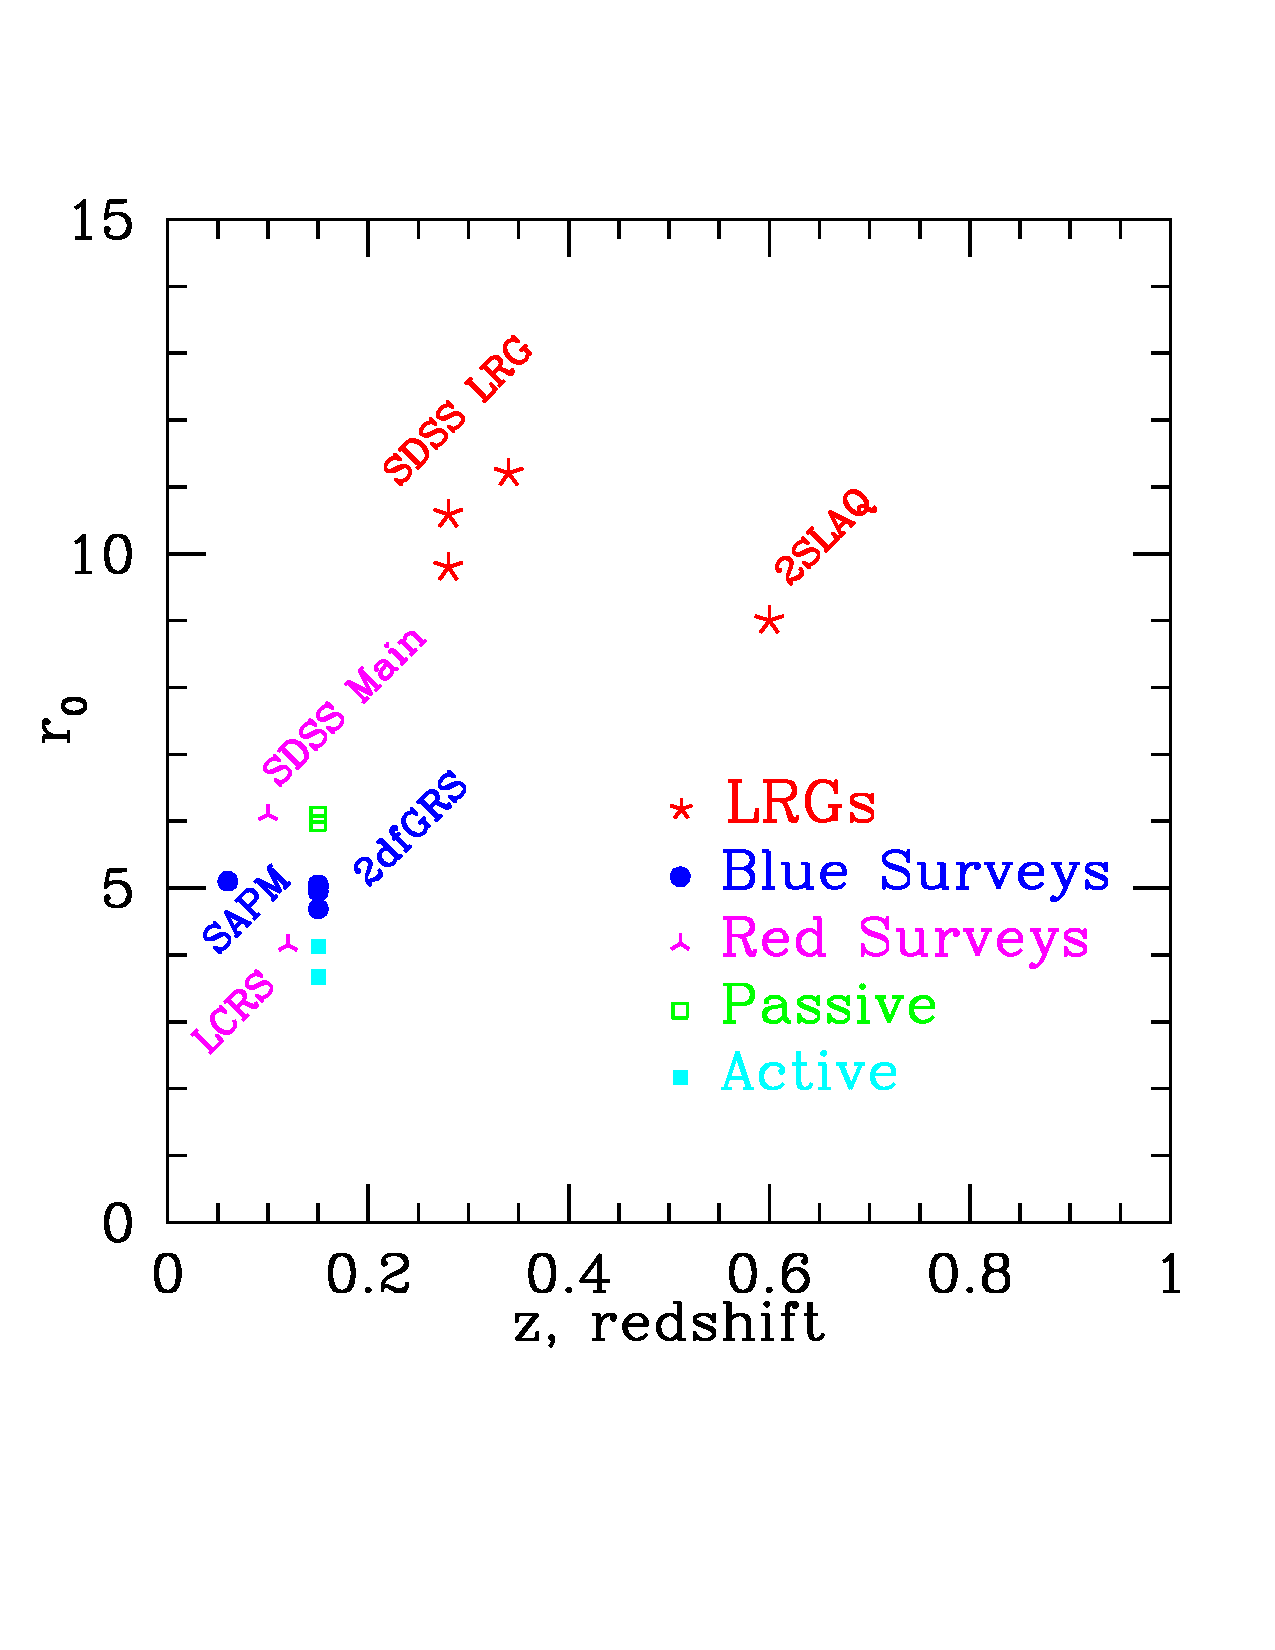
\includegraphics[height=8.0cm,width=8.0cm]
                  {pdf/r_nought_z_labels.pdf}
  \centering
  \caption[A comparisson of the real-space correlation length, $r_{0}$ between various surveys]
          {A comparisson of the real-space correlation length, $r_{0}$ between various surveys. 
           Note that this should only be taken as a guide 
           as different surveys have differnet galaxy selection criteria 
           and sample different populations. 
           Care has to taken even when comparing the 2SLAQ and SDSS LRG surveys.}
  \label{fig:r_nought_z_labels}
\end{figure}


\begin{figure}
  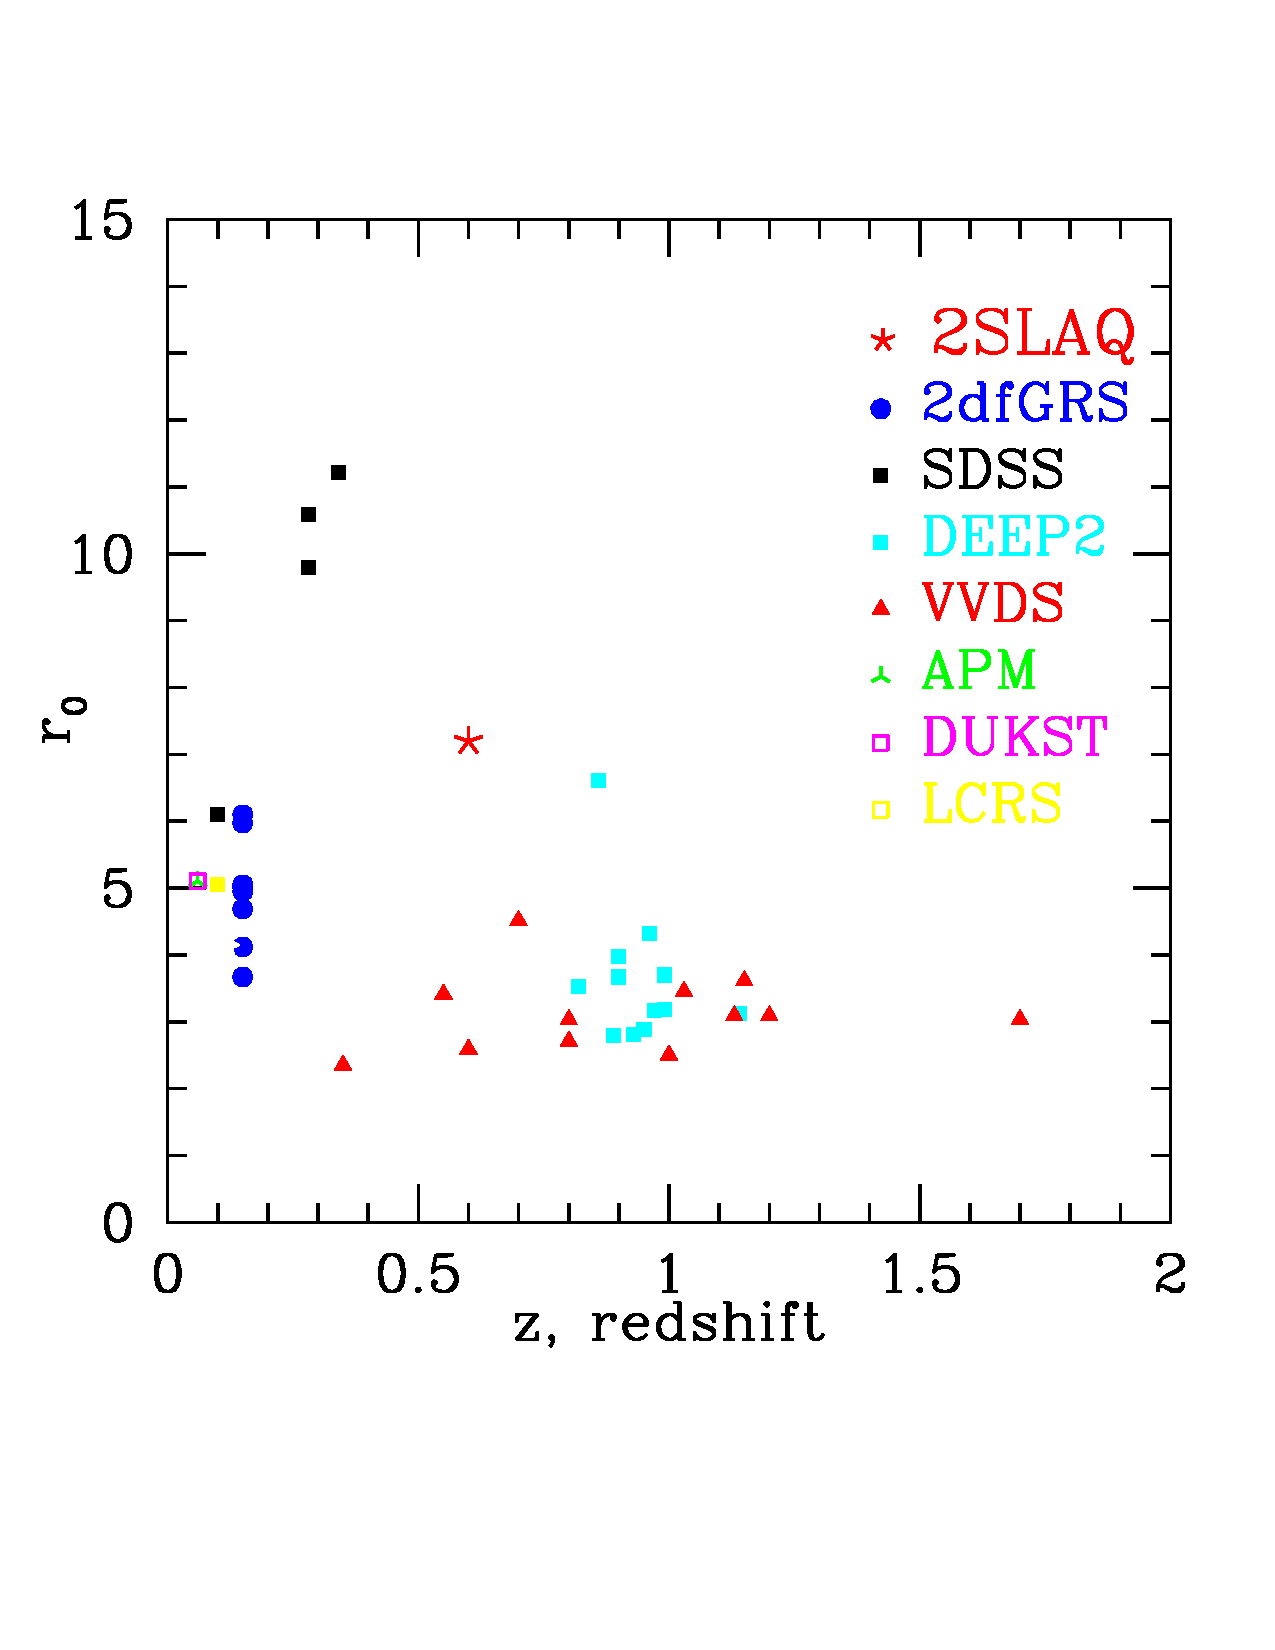
\includegraphics[height=8.0cm,width=8.0cm]{pdf/r_nought_z.pdf}
  \centering
  \caption{A further comparisson of the real-space correlation length, 
    $r_{0}$ between various surveys. 
    Again care must be taken as comparing ``wide and shallow'' to ``deep and
    narrow''. For instance the areas of the 2dfGRS and SDSS 
    are 1 800 and 4 000 degrees$^{2}$ respectively, while COMBO-17, 
    DEEP2 and VVDS are of order 1 degree$^{2}$.}
  \label{fig:r_nought_z}
\end{figure}




\begin{table*}
\baselineskip=20pt
\begin{center}
\setlength{\tabcolsep}{1pt}
\begin{tabular}{llcccrccc}
\hline
\hline
Survey            &   Sample\,\,\,  & $z$-interval &  median $z$     & Mag. limit & $N_{\rm gals}$ & $r_{0}$  & $\gamma_{r}$  & Reference   \\
%Have, instead of a mag limit, a L/L* number?? (as in Madgwick, table 3??) Could also have a ``Survey Mag limit'' thing
% i.e. the L/L* tells you info about the luminosity of the survey while, the survey amg limit basically says red or blue?!?
% WHAT ABOUT A COLUMN FOR AREA???
\hline
\hline
2SLAQ LRG     & full                &0.4,0.8    & 0.55           &                          &    9 816 &  7.20$^{+0.8}_{-1.0}$ & 1.80$^{+0.18}_{-0.22}$   &\\
\hline
SDSS LRG$^1$  & ``full, faintest''  &0.16,0.36  & 0.28           & $-23.2< M_{g} < -21.20$, $\langle M_{g}\rangle=-21.63$ &   29 298 &  9.80$\pm$0.20 & 1.94$\pm$0.03   & \\
SDSS LRG$^1$  & ``brighter half''   &0.16,0.44  & 0.34           & $-23.2< M_{g} < -21.8 $, $\langle M_{g}\rangle=-22.01$ &   12 992 & 11.21$\pm$0.24 & 1.92$\pm$0.03   & \\
SDSS LRG$^1$  & ``fainter half''    &0.16,0.36  & 0.28           & $-22.6< M_{g} < -21.6 $, $\langle M_{g}\rangle=-21.84$ &   14 500 & 10.59$\pm$0.29 & 1.88$\pm$0.03   &  \\
\hline
SDSS MAIN$^2$ & &0.,0.      &                &                          &          &                       &             &             \\
\hline 
VVDS$^3$      &         &0.,0.      &                &                          &          &                       &             &             \\
%VVDS-02h     & 	&[0.2-0.5] 	1277  -17.57  1.34	2.35_{-0.37}^{+0.36}	1.78_{-0.08}^{+0.11} 	2.27 0.29
%VVDS-02h     & 	&[0.5-0.7] 	1461  -18.68  1.28	2.59_{-0.39}^{+0.37} 	1.66_{-0.08}^{+0.12} 	2.61 0.41
%VVDS-02h     &		&[0.7-0.9] 	1428  -19.20  1.36 	2.71_{-0.36}^{+0.39} 	1.57_{-0.07}^{+0.10} 	2.69 0.43
%VVDS-02h     & 	&[0.9-1.1] 	1034  -19.66  1.35 	2.50_{-0.39}^{+0.39} 	1.57_{-0.08}^{+0.11} 	2.35 0.51
%VVDS-02h     &		&[1.1-1.3] 	 571  -20.26  1.35 	3.09_{-0.53}^{+0.52} 	1.85_{-0.17}^{+0.22}  	2.93 0.66 \\
%VVDS-02h     &		&[1.3-2.1] 	 436  -20.93  1.25 	3.03_{-0.56}^{+0.51} 	1.45_{-0.12}^{+0.17} 	3.30 1.20 \\
%VVDS-02h DEEP2 selectn	&[0.7-1.35] 	1620  -20.00  1.36 	3.45_{-0.67}^{+0.55} 	1.63_{-0.09}^{+0.12} 	3.51 0.63 \\
%VVDS-02h DEEP2 selectn	&[0.7-0.9] 	 687  -19.65  1.41 	3.03_{-0.58}^{+0.56} 	1.49_{-0.09}^{+0.135} 	3.37 0.67 \\
%VVDS-02h DEEP2 selectn & [0.9-1.35] 	 933  -20.25  1.32 	3.09_{-0.41}^{+0.43} 	1.68_{-0.10}^{+0.12} 	3.05 0.47 \\
%VVDS-CDFS		&[0.4-0.7] 	 421  -19.44  1.30 	3.41_{-0.85}^{+0.78} 	1.42_{-0.14}^{+0.20} 	3.53_{-1.00}^{+0.73} \\
%VVDS-CDFS 		&[0.6-0.8] 	 372  -19.74  1.47 	4.51_{-1.06}^{+0.97} 	1.59_{-0.20}^{+0.25} 	4.31 1.16\\
%VVDS-CDFS 		&[0.8-1.5] 	 452  -20.43  1.34 	3.61_{-1.05}^{+1.22} 	1.68_{-0.27}^{+0.29} 	3.63 0.89\\
\hline
DEEP2$^4$     &full &0.7,1.35   & $z_{\rm eff}=0.99$ & $R_{AB}$=24.1            &    2 219 & $3.19\pm$0.51         & 1.68$\pm$0.07 &           \\
DEEP2$^4$     &full, w/o $J_{3}$ &0.7,1.35   & $z_{\rm eff}=0.99$ & $R_{AB}$=24.1            &    2 219 & $3.19\pm$0.51         & 1.68$\pm$0.07  &          \\
DEEP2$^4$     &lower-$z$ &0.7,1.35   & $z_{\rm eff}=0.99$ & $R_{AB}$=24.1            &    2 219 & $3.19\pm$0.51         & 1.68$\pm$0.07  &          \\
DEEP2$^4$     &higher-$z$ &0.7,1.35   & $z_{\rm eff}=0.99$ & $R_{AB}$=24.1            &    2 219 & $3.19\pm$0.51         & 1.68$\pm$0.07  &          \\
DEEP2$^4$     & $(B-R)>0.7$ &0.7,1.25   & $z_{\rm eff}=0.96$ & $(B-R)_0 >0.7$           &      855 & $4.32\pm$0.73         & 1.84$\pm$0.07     &       \\
DEEP2$^4$     & $(B-R)<0.7$ &0.7,1.25   & $z_{\rm eff}=0.93$ & $(B-R)_0 <0.7$           &      964 & $2.81\pm$0.48         & 1.52$\pm$0.06   &         \\
DEEP2$^4$     & $(R-I)>0.9$ &0.7,1.25   & $z_{\rm eff}=0.96$ & $(B-R)_0 >0.7$           &      855 & $4.32\pm$0.73         & 1.84$\pm$0.07     &       \\
DEEP2$^4$     & $(R-I)>0.09$ &0.7,1.25   & $z_{\rm eff}=0.96$ & $(B-R)_0 >0.7$           &      855 & $4.32\pm$0.73         & 1.84$\pm$0.07     &       \\
DEEP2$^4$     & absorption-line &0.7,1.25   & $z_{\rm eff}=0.96$ & $(B-R)_0 >0.7$           &      855 & $4.32\pm$0.73         & 1.84$\pm$0.07     &       \\
DEEP2$^4$     & emission-line &0.7,1.25   & $z_{\rm eff}=0.96$ & $(B-R)_0 >0.7$           &      855 & $4.32\pm$0.73         & 1.84$\pm$0.07     &       \\
DEEP2$^4$     & $M_{B}<-19.75$ &0.7,1.25   & $z_{\rm eff}=0.96$ & $(B-R)_0 >0.7$           &      855 & $4.32\pm$0.73         & 1.84$\pm$0.07     &       \\
DEEP2$^4$     & $M_{B}>-19.75$ &0.7,1.25   & $z_{\rm eff}=0.96$ & $(B-R)_0 >0.7$           &      855 & $4.32\pm$0.73         & 1.84$\pm$0.07     &       \\

\hline
2dfGRS$^5$    & Full, (P)    &0.01,0.2   & $\simeq$ 0.11  & $\bj$ = 19.45            &  165 659 & $5.05\pm$0.26         & 1.67$\pm$0.03   &         \\
2dfGRS$^5$    & Full, (I)    &0.01,0.2   & $\simeq$ 0.11  & $\bj$ = 19.45            &  165 659 & $5.05\pm$0.26         & 1.67$\pm$0.03   &         \\
\hline
2dfGRS$^6$    & Full, (P)    &0.01,0.2   & $\simeq$ 0.11  & $\bj$ = 19.45            &  165 659 & $5.05\pm$0.26         & 1.67$\pm$0.03   &         \\
2dfGRS$^6$    & Full, (I)    &0.01,0.2   & $\simeq$ 0.11  & $\bj$ = 19.45            &  165 659 & $5.05\pm$0.26         & 1.67$\pm$0.03   &         \\
2dfGRS$^6$    & Passive, (P) &0.01,0.15  & $z_{\rm s}= 0.11$  & $\bj$ = 19.45            &   36 318 & $5.97\pm$0.29         & 1.93$\pm$0.03 &           \\
2dfGRS$^6$    & Passive, (I) &0.01,0.15  & $z_{\rm s}= 0.11$  & $\bj$ = 19.45            &   36 318 & $5.97\pm$0.29         & 1.93$\pm$0.03  &          \\
2dfGRS$^6$    & Active, (P)  &0.01,0.15  & $z_{\rm s}= 0.11$  & $\bj$ = 19.45            &   60 473 & $7.1 \pm$0.1          & 1.50$\pm$0.04  &          \\
2dfGRS$^6$    & Active  (P)  &0.01,0.15  & $z_{\rm s}= 0.11$  & $\bj$ = 19.45            &   60 473 & $7.1 \pm$0.1          & 1.50$\pm$0.04  &          \\
\hline
SAPM          & &0.01,0.15  & $z_{\rm s}= 0.11$  & $\bj$ = 19.45            &   60 473 & $7.1 \pm$0.1          & 1.50$\pm$0.04 &           \\
ESP           & &0.01,0.15  & $z_{\rm s}= 0.11$  & $\bj$ = 19.45            &   60 473 & $7.1 \pm$0.1          & 1.50$\pm$0.04 &          \\
Durham UKST   & &0.01,0.15  & $z_{\rm s}= 0.11$  & $\bj$ = 19.45            &   60 473 & $7.1 \pm$0.1          & 1.50$\pm$0.04 &           \\
LCRS          & &0.01,0.15  & $z_{\rm s}= 0.11$  & $\bj$ = 19.45            &   60 473 & $7.1 \pm$0.1          & 1.50$\pm$0.04 &           \\
%SDSS from Hawkins03
\hline
\hline
\end{tabular}
\caption[Comparison of Real-Space Correlation Lengths with other surverys.]
{Comparison of Real-Space Correlation Lengths with other surverys.
  $^1$Zehavi et al. 2005a, $^2$Zehavi et al. 2005b, $^3$Pollo et al. 2004, $^4$Coil. et al. 2004, $^5$Hawkins et al. 2003, 
  $^6$Magdwick et al. 2003. 
%Note, used the Inverted Methods for 2SLAQ and 2dFGRS figures...
%For Hawkings, the z_median is \simeq 0.11, while the ``effective survey'' z=0.15
%Madgwich only quotes (I think) the ``effective survey'' z, which is 0.11 for all three of their samples
%Also the Mag limit for 2dFGRS might well have changed since these papers, better see Cole et al. for latest no...???
}
\label{tab:r_nought_comp}

\end{center}
\end{table*}



\section{Notes}
LBGs Adelberger, Steidel et al etc. 
Blain, quoting Overtier 03, A\&A, 405, 53


DRGs
EROs Kong, Almani?
SMGs Blain

Go back to the .sm plots and put on the 
Simple xi(r) evolution model(s) from Croom et al. (??!)

$\xi(r) = \frac{r}{r_{0}}^{-\gamma + \epsilon}$ what's the tag for the ``euro'' sign/symbol that goes in this equation?!?!?
(heck, that small ``slash epsilon'' tag seems to work fine!

{\LARGE ALSO!!! }


M$_{\rm halo}$ MODELS vs. redshift ... 
e.g. 


{\bf Farrah, D et al.,  2006 ApJ  643L 139} and 
{\bf Farrah, D et al.,  2006 ApJ  641, L17}.  
Comoving correlation length, r0, vs. redshift. Other data are taken from Moscardini et al. (1998), Overzier et al. (2003), Daddi et al. (2004), Blain et al. (2004), Ouchi et al. (2004), Adelberger et al. (2005), Croom et al. 2005; Georgakakis et al. (2005), and Allen et al. (2005). The fixed mass lines show the predicted clustering amplitude of halos of a given mass at any particular redshift, whereas the $\epsilon$ lines show the predicted clustering amplitude of an individual halo for three halo growth models, described in the text. The stable and linear lines give a qualitative indicator of the range of how DM halos may grow with redshift, and we have normalized stable and linear lines to the clustering amplitudes of the B2 and B3 sources. The shaded regions therefore indicate what these halos may host at lower and higher redshifts the halos hosting B3 sources may contain an optically bright LBG at z $\simeq$ 4 (upper green circle) and may grow to host very rich galaxy clusters at z = 0, whereas the halos hosting B2 sources may contain optically fainter LBGs at $4 < z < 5$, SMGs at z $sim$ 2.5, radio-bright AGNs (upper pink triangle) and (old) EROs at z $\simeq$ 1, and poor to rich clusters at z = 0.

{\bf Hayashi et al. astro-ph/0701637.pdf} - for star-forming BzKs...




\section{$\Omega_{\rm m}-\beta$ fitting models}

\begin{table*}
\begin{center}
\caption{}
\setlength{\tabcolsep}{1pt}
\begin{tabular}{lccccccccc}
\hline
\hline
O/P file name  &   I/P $\xisp$ files                  &  r0  & $\gamma$ &  range    &  $\xi/w_p$ & $\Omm$ & beta & $\wrms$ & R$\chi^2$ \\

\hline
LS\_amp7\_3.ps & k2d\_output\_jack\_perl\_full.dat??? &	7.30 & 1.78      &  0.4-70(?) & $\xi$   &  0.30  & 0.35 & 480  & \\ 
               & xi\_sigma\_pi\_variances\_LS.dat???  &      &           &            &         &        &      &      & \\[8pt]
%
%
LS\_amp8\_3.ps & tbc                                  & 7.54 & 1.85      & 0.4-20     & $w_p$  &  0.50  & 0.45 & 540  & \\
               & tbc                                  &      &           &            &         &        &      &      & \\[8pt]
%
%
LS\_amp9\_3.ps & k2d\_output\_jack\_perl\_full.dat    & 7.45 & 1.73      & 0.4-70     & $\xi$   &  0.50	 & 0.35	& 450  & 2.14920  \\
(0.3,0.7) y/n? & xi\_sigma\_pi\_variances\_LS.dat     &      &           &            &         &        &      &      &          \\[8pt]
%
%
LS\_amp10\_3.ps & k2d\_output\_jack\_perl\_full\_newcor.dat & 7.45 &  1.73 & 0.4-70   & $\xi$	& 0.45	& 0.35	& 450	& 2.18665 \\
(0.3,0.7) y/n?  & xi\_sigma\_pi\_variances\_LS.dat          &      &       &          &         &       &       &       &         \\
%
LS\_ampX3\_3.ps	& ''                                        & 7.45          & 1.73    & 0.4-70   & xi      & 0.10  & 0.40 & 330  &  2.19586 \\
		& Omega\_m\_StdDev                          &  0.024552442  &         &          &         &       &      &      & \\
		& beta\_StdDev                              &  0.0088388369 &         &          &         &       &      &      & \\
%
LS\_ampRX0.ps   & (reduced range in Omega-beta)             &               &         &          &         &       &      &      & \\[8pt]
%
%
LS\_amp11\_3.ps	& k2d\_output\_jack\_perl\_full\_newcor.dat & 7.45          & 1.73 &  0.4-70 & $\xi$ & 0.45  & 0.35  & 450  & 2.18665 \\
(0.3,0.7) y/n?  & xi\_sigma\_pi\_variances\_LS.dat          &               &      &         &       &       &       &      & \\
%
LS\_ampX5\_3.ps	&                                           & 7.30          & 1.84 &  0.4-70 & $w_p$ & 0.02  & 0.40  & 360  &  2.26280\\
		& Omega\_m\_StdDev                          & 0.068530072   &      &         &       &       &       &      & \\
		& beta\_StdDev                              & 0.028398096   &      &         &       &       &       &      & \\[8pt]
%
%
LS\_amp12\_3.ps	& k2d\_output\_jack\_perl\_full\_newcor.dat & 7.60          & 1.69 &  0.4-20 & xi   & 0.40   & 0.30 & 420  & 2.35397 \\
(0.3,0.7) y/n?  & xi\_sigma\_pi\_variances\_LS.dat          &               &      &         &      &        &      &      & \\
%
LS\_ampX6\_3.ps	&                                           & 7.60          & 1.69 &  0.4-20 & xi   & 0.10   & 0.35 & 300  &	2.35562 \\
		& Omega\_m\_StdDev                          & 0.051742808   &      &         &      &        &      &      & \\
		& beta\_StdDev                              & 0.027679029   &      &         &      &        &      &      & \\[8pt]
%
%
LS\_amp13\_3.ps	& k2d\_output\_jack\_perl\_full\_newcor.dat &  7.39         & 1.81 &  0.4-20 & wp   & 0.65  & 0.45  & 510  & 2.16416 \\
                & xi\_sigma\_pi\_variances\_LS.dat          &               &      &         &      &       &       &      & \\
(1.0,0.0)$^1$   &                                           &               &      &         &      &       &       &      & \\
%
LS\_ampX4\_3.ps	&                                           &  7.39         & 1.81 &  0.4-20 & wp   & 0.10  & 0.45  & 360  & 2.16491 \\[8pt]
%
%
LS\_ampX\_3.ps  & k2d\_output\_jack\_perl\_full\_newcor.dat & 7.54	    & 1.85 &  0.4-20 & wp   & 0.65  & 0.50  & 540  & 2.32433 \\
(0.3,0.7) y/n?  & xi\_sigma\_pi\_variances\_LS\_0606016.dat &               &      &         &      &       &       &      & \\[8pt]
%
LS\_ampX2\_3.ps & k2d\_output\_jack\_perl\_full\_newcor.dat & 7.54	    & 1.85 &  0.4-20 & wp   & 0.65  & 0.50  & 540  & 2.29314 \\
(0.3,0.7) y/n?	& xi\_sigma\_pi\_variances\_LS.dat          &               &      &         &      &       &       &      & \\[16pt]
%
%	
\hline
%
LS\_amp6\_EdS\_3.ps  & k2d\_output\_jack\_perl\_EdS\_full.dat  & 5.60         & 1.71  & 0.25-40 &  xi  & 0.40  & 0.45  & 330  & 2.22507 \\
(1.0,0.0) y/n?	     &  xi\_sigma\_pi\_variances\_LS\_EdS.dat  &              &       &         &      &       &       &      & \\[8pt]

LS\_ampX6\_EdS\_3    &                                         &  5.60	      & 1.71  & 0.25-40 &  xi  & 0.50  & 0.50  & 330  & 2.37068 \\
LS\_ampXX6\_EdS\_3   & 	                                       &  5.60	      & 1.71  & 0.25-40 &  xi  & 0.40  & 0.45  & 330  & 2.22507 \\
                     & (LS\_amp6 identical to LS\_ampXX6)      &              &       &         &      &       &       &      & \\
		     & Omega\_m\_StdDev                        &  0.14701328  &       &         &      &       &       &      & \\
		     & beta\_StdDev                            &  0.033261847 &       &         &      &       &       &      & \\[8pt]
%
%
LS\_amp8\_EdS\_3.ps  & k2d\_output\_jack\_perl\_EdS\_full.dat  & 5.61         & 1.77  &  0.25-40 &  wp & 0.45  & 0.50  & 360  & 1.91541\\
(1.0,0.0) y/n?	     & xi\_sigma\_pi\_variances\_LS\_EdS.dat   &              &       &          &     &       &       &      & \\[8pt]
%	
LS\_ampX8\_EdS\_3    &                                         & 5.61         & 1.77  &  0.25-40 &  wp & 0.45  & 0.50  & 360  & 1.91541 \\[8pt]
%
%
LS\_amp9\_EdS\_3.ps  & k2d\_output\_jack\_perl\_EdS\_full.dat  & 5.55         & 1.73  &  0.25-15 &  xi & 0.40  & 0.50  & 360  & 2.09865\\
		     &   xi\_sigma\_pi\_variances\_LS\_EdS.dat &              &       &           &     &       &       &      & \\[8pt]
%
%
LS\_amp10\_EdS\_3.ps & k2d\_output\_jack\_perl\_EdS\_full.dat  & 5.67         & 1.74  & 0.25-15  &  wp &       &       &      & \\
		     & xi\_sigma\_pi\_variances\_LS\_EdS.dat   &              &       &          &     &       &       &      & \\[8pt]
%
%
LS\_amp7\_EdS\_3.ps  & k2d\_output\_jack\_perl\_EdS\_full.dat  & 5.55         & 1.735 &   0.1-15 &  xi &  0.40 & 0.50  & 360  &  2.06925 \\
		     & xi\_sigma\_pi\_variances\_LS\_EdS.dat   &              &       &          &     &       &       &      & \\[8pt]
\hline
\hline
\label{}
\end{tabular}
\end{center}
\end{table*}
$^1$Is this really correct??


\begin{table*}
\centering
\caption{Best fitting model values of $\Omm, \beta$ and 
pairwise velocity dispersion, $\wrms$, 
using redshift-space distortions alone and assuming a $\Lambda$CDM cosmology.}
\begin{tabular}{||l|c|c|c|l|c|c} \hline
\hline
r$_{0}$ & $\gamma$ &  range /$\hmpc$ & Measure & $\Omm$ & $\beta$ & $\wrms / \kms$ \\
\hline
7.45     &  1.73    &  0.4-70        & $\xir$  &   0.10 &  0.40   &  330    \\
7.30     &  1.84    &  0.4-70	     & $\wp $  &   0.02 &  0.40   &  360    \\
7.60     &  1.69    &  0.4-20        & $\xir$  &   0.10 &  0.35   &  300    \\
7.39     &  1.81    &  0.4-20        & $\wp$   &   0.10 &  0.45   &  360    \\
\hline
\end{tabular}
\label{tab:zspace_dist_values}
\end{table*}

%Lambda
%.4 - 70 Mpc h^-1  xi(r)               7.45     1.73    amp10, ampX3
%.4 - 70 Mpc h^-1  wp(sigma)           7.30     1.84    amp11, ampX5   
%.4 - 20 Mpc h^-1  xi(r)               7.60     1.69    amp12, ampX6   
%.4 - 20 Mpc h^-1  wp(sigma)           7.39     1.81    amp13, ampX4    

%EdS
%.25 - 40 Mpc h^-1  xi(r)              5.60     1.71    amp6   
%.25 - 40 Mpc h^-1  wp(sigma)          5.61     1.77    amp8
%.25 - 15 Mpc h^-1  xi(r)              5.55     1.73    amp9    
%.25 - 15 Mpc h^-1  wp(sigma)          5.67     1.74    amp10   run.



%As of Aug 07 09:54:
%/cos/pc19a/npr/programs/jaca\_xisp\_Omegam\_beta/xisp\_fitting > ll *k2d*ful*
%-rw-r--r--  1 npr dphcosm 56778 Jul  7 10:12 k2d\_output\_jack\_perl\_full\_EdS\_070706.dat
%-rw-r--r--  1 npr dphcosm 56790 Jul 11 16:24 k2d\_output\_jack\_perl\_full.dat
%-rw-r--r--  1 npr dphcosm 56790 Jul 11 16:24 k2d\_output\_jack\_perl\_full\_nocor.dat
%-rw-r--r--  1 npr dphcosm 56794 Jul 11 16:24 k2d\_output\_jack\_perl\_full\_newcor\_110706.dat
%-rw-r--r--  1 npr dphcosm 56698 Jul 19 10:48 k2d\_output\_jack\_perl\_EdS\_full.dat
%-rw-r--r--  1 npr dphcosm 56790 Jul 19 15:10 k2d\_output\_jack\_perl\_full\_newcor.dat

%/cos/pc19a/npr/programs/jaca\_xisp\_Omegam\_beta/xisp\_fitting > ll *vari*
%-rw-r--r--  1 npr dphcosm 4870 Jun 16 10:00 xi\_sigma\_pi\_variances\_LS\_0606016.dat
%-rw-r--r--  1 npr dphcosm 4846 Jul  7 10:10 xi\_sigma\_pi\_variances\_LS\_EdS\_070706.dat
%-rw-r--r--  1 npr dphcosm 5314 Jul 19 11:14 xi\_sigma\_pi\_variances\_LS\_EdS.dat
%-rw-r--r--  1 npr dphcosm 4853 Jul 19 18:16 xi\_sigma\_pi\_variances\_LS.dat



\end{document}
